%-----------------------------------------------------------------------------%
\chapter{\babLima}
%-----------------------------------------------------------------------------%


\newcommand\MyHead[2]{%
	\multicolumn{1}{l}{\parbox{#1}{\centering #2}}
}


%-----------------------------------------------------------------------------%
\section{Implementasi}
\label{sec:implementation}
%-----------------------------------------------------------------------------%
Algoritma yang dirancang pada \autoref{sec:design} diimplementasikan dengan menggunakan beberapa bahasa pemrograman yang kemudian dikombinasikan dengan aplikasi pihak ketiga untuk menghasilkan sebuat prototipe. Subbab ini akan berisi penjabaran lengkap tentang implementasi sistem. 


%-----------------------------------------------------------------------------%
\subsection{\textit{VRP Solver}}
%-----------------------------------------------------------------------------%

\textit{VRP Solver} yang telah dirancang pada \autoref{ssec:vrp-solver} diimplementasikan dalam bahasa pemrograman C++. C++ dipilih karena memiliki manajemen \textit{resources} (\textit{processor} dan \textit{memory}) yang lebih efisien dibandingkan bahasa pemrograman lainnya, sehingga dinilai tepat untuk menangani permasalahan kombinatorial VRP yang membutuhkan komputasi yang intensif. 

\textit{Source code VRP Solver} tersedia dan dapat diunduh pada pada tautan: \url{https://github.com/soedomoto/coes-mdvrp/tree/jni-coes-mdvrp}. \textit{VRP Solver} diimplementasikan dan dikompilasi di dalam lingkungan berikut:
\begin{itemize}
	\item Sistem Operasi		: Elementary OS Loki (Berbasis Ubuntu 16.04)
	\item C++ Compiler			: c++ (Ubuntu 5.4.0-6ubuntu1~16.04.4) 5.4.0 20160609
	\item Hardware				: Asus TP300L, Quad-Core Intel® Core™ i3-4030U CPU @ 1.90GHz, 3,7 GiB DDRIII, 256GB SSD
\end{itemize}


%-----------------------------------------------------------------------------%
\subsection{\textit{Publisher} Rekomendasi}
%-----------------------------------------------------------------------------%
\textit{Publisher} rekomendasi yang tersusun atas \autoref{alg:topic-watcher} dan \autoref{alg:vrp-worker} diimplementasikan dalam bahasa pemrograman Python. Python merupakan \textit{interpreter language} dengan struktur \textit{syntax} yang simpel sehingga mudah untuk digunakan dalam penyusunan prototipe. Lingkungan yang digunakan dalam implementasi \textit{publisher} rekomendasi adalah sebagai berikut:

\begin{itemize}
	\item Sistem Operasi		: Elementary OS Loki (Berbasis Ubuntu 16.04)
	\item Python version		: Python 2.7.12
	\item Hardware				: Asus TP300L, Quad-Core Intel® Core™ i3-4030U CPU @ 1.90GHz, 3,7 GiB DDRIII, 256GB SSD
\end{itemize}

\textit{Source code} dari \textit{publisher} rekomendasi dapat diunduh di: \url{https://github.com/soedomoto/coes-mdvrp/tree/py-mdvrp-producer-redis}

%-----------------------------------------------------------------------------%
\section{Pengujian}
\label{sec:testing}
%-----------------------------------------------------------------------------%
Pengujian dilakukan untuk mengetahui tingkat ketercapaian tujuan penelitian ini yang meliputi:
\begin{itemize}
	\item Perancangan algoritma \textit{publisher} yang dapat memberikan rekomendasi terbaik secara global.
	\item Penyusunan mekanisme \textit{conflict resolution} untuk menghindari terjadinya rekomendasi lokasi yang sama pada dua atau lebih pencacah.
\end{itemize}

Akurasi algoritma diukur dengan cara membandingkan hasil pengujian sistem usulan dengan hasil pengujian algoritma MDVRP berbasis CoEAs tanpa mekanisme \textit{publish/subscribe}.


%-----------------------------------------------------------------------------%
\subsection{Lingkungan Pengujian}
\label{ssec:test-environment}
%-----------------------------------------------------------------------------%
Pengujian sistem rekomendasi lokasi dilakukan di dalam lingkungan sebagai berikut:
\begin{itemize}
	\item Sistem Operasi		: Elementary OS Loki (Berbasis Ubuntu 16.04)
	\item Redis Environment		: Redis 3.2.6, Debian Jessie (Docker version)
	\item Python version		: Python 2.7.12
	\item Hardware				: Asus TP300L, Quad-Core Intel® Core™ i3-4030U CPU @ 1.90GHz, 3,7 GiB DDRIII, 256GB SSD
\end{itemize}


%-----------------------------------------------------------------------------%
\subsection{\textit{Dataset} dan \textit{Metric}}
%-----------------------------------------------------------------------------%
%-----------------------------------------------------------------------------%
\subsubsection{\textit{Dataset}}
%-----------------------------------------------------------------------------%
Berbagai variasi data digunakan untuk memastikan validitas pengujian. Pengujian terkait \textit{Vehicle Routing Problem} umumnya dilakukan dengan memanfaatkan data Breedam, Cordeau, Solomon, Homberger, dan Russell. Data Cordeau mengandung 8 (delapan) tipe VRP \textit{problem}, sebagai berikut:

\begin{enumerate}
	\item Tipe 0 untuk kasus VRP
	\item Tipe 1 untuk kasus Periodic VRP
	\item Tipe 2 untuk kasus Multi-Depot VRP
	\item Tipe 3 untuk kasus Split Delivery VRP
	\item Tipe 4 untuk kasus VRP dengan Time Windows
	\item Tipe 5 untuk kasus Periodic VRP dengan Time Windows
	\item Tipe 6 untuk kasus Multi-Depot VRP dengan Time Windows
	\item Tipe 7 untuk kasus Split Delivery VRP dengan Time Windows
\end{enumerate}

Pada penelitian ini, pengujian dilakukan dengan menggunakan dataset Cordeau tipe 2 (Multi-Depot VRP), dengan struktur format sebagai berikut:
\begin{enumerate}
	\item Baris pertama berformat \textbf{TYPE M N T}, dengan: \\
	M = Jumlah kendaraan \\
	N = Jumlah pelanggan \\
	T = Jumlah \textit{depot}
	
	\item Baris kedua sampai T baris berikutnya berformat \textbf{D Q}, dengan: \\
	D = Durasi maksimum dari setiap rute \\
	Q = Kapasitas maksumum dari setiap kendaraan
	
	\item Baris selanjutnya sampai M baris berikutnya berformat \textbf{i x y d q f a list e l}, dengan: \\
	i	= nomer pelanggan \\
	x	= koordinat x \\
	y	= koordinat y \\
	d	= durasi pelayanan (\textit{service time}) \\
	q	= \textit{demand} \\
	f	= frekuensi kunjungan \\
	a	= jumlah kombinasi kunjungan \\
	list	= list dari semua kombinasi kunjungan \\
	e	= jika ada, waktu dimulainya kunjungan \\
	l	= jika ada, waktu selesainya kunjungan
	
	\item Baris selanjutnya sampai M baris berikutnya berformat \textbf{i x y}, dengan: \\
	i	= nomer kendaraan \\
	x	= koordinat depot x \\
	y	= koordinat depot y \\
\end{enumerate}

Untuk menyimulasikan kondisi lapangan yang sebenarnya, sistem juga diuji dengan menggunakan data lapangan wilayah administratif di Kabupaten Pesisir Selatan, Provinsi Sumatera Barat. Data lapangan digunakan untuk merepresentasikan kondisi pencacahan yang sebenarnya, dengan antar lokasi terdapat \textit{cost} yang berupa jarak dan waktu tempuh.

Data lapangan yang digunakan meliputi:
\begin{itemize}
	\item data 182 lokasi pencacahan beserta posisi koordinatnya yang dianalogikan sebagai pelanggan (N = 182). 
	\item data 15 petugas pencacahan yang dianalogikan sebagai kendaraan ($M$ = 15) beserta koordinat \textit{initial depot} tiap-tiap pencacah.
\end{itemize}

Untuk setiap kombinasi lokasi pencacahan dan \textit{initial depot} dari petugas, dilakukan penghitungan waktu tempuhnya dengan memanfaatkan \textit{Google Direction API}, sebagaimana dijelaskan pada \autoref{ss:distance-duration-matrix}.


%-----------------------------------------------------------------------------%
\subsubsection{\textit{Metric}}
\label{sssec:metric}
%-----------------------------------------------------------------------------%
Sistem usulan yang menggunakan algoritma MDVRP berbasis CoEAs dan mekanisme \textit{publish/subscribe} akan dibandingkan dengan program pembanding yang menggunakan algoritma yang sama, namun tanpa mekanisme \textit{publish/subscribe}. Tiap-tiap pengujian akan menghasilkan output berupa rute untuk setiap petugas pencacahan seperti contoh berikut:

\begin{itemize}
	\item \textit{Vehicle} A = Loc1 $\rightarrow$ Loc5 $\rightarrow$ Loc15 $\rightarrow$ Loc12
	\item \textit{Vehicle} B = Loc 6 $\rightarrow$ Loc2 $\rightarrow$ Loc16 $\rightarrow$ Loc3
	\item \textit{Vehicle} C = Loc4 $\rightarrow$ Loc8 $\rightarrow$ Loc14 $\rightarrow$ Loc 7
	\item \textit{Vehicle} D = Loc9 $\rightarrow$ Loc10 $\rightarrow$ Loc11 $\rightarrow$ Loc12
\end{itemize}


\begin{figure}[!]
	\centering
	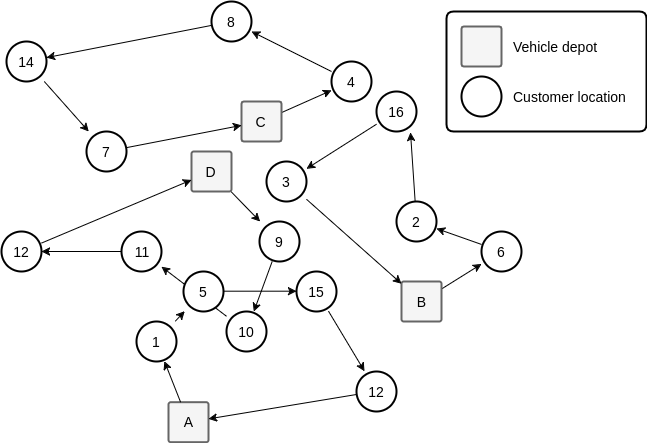
\includegraphics[width=9cm]{Resources/Images/result-mdvrp-illustration}
	\captionsetup{format=hang}
	\caption{Ilustrasi Rute yang Dihasilkan}
	\label{fig:result-mdvrp-illustration}
\end{figure}


Biaya total untuk tiap-tiap rute kemudian dihitung dengan melakukan penjumlahan seluruh waktu tempuh dan waktu pelayanan (\textit{service time}) dari lokasi yang dikunjungi. Pada contoh \autoref{fig:result-mdvrp-illustration}, biaya total dari setiap kendaraan adalah:

\begin{itemize}
	\item $TC_A$ = $C_{A-1}$ + $ST_5$ + $C_{1-5}$ + $ST_5$ + $C_{5-15}$ + $ST_15$ + $C_{15-12}$ + $ST_12$ + $C_{12-A}$
	\item $TC_B$ = $C_{B-6}$ + $ST_6$ + $C_{6-2}$ + $ST_2$ + $C_{2-16}$ + $ST_16$ + $C_{16-3}$ + $ST_3$ + $C_{3-B}$
	\item $TC_C$ = $C_{C-4}$ + $ST_4$ + $C_{4-8}$ + $ST_8$ + $C_{8-14}$ + $ST_14$ + $C_{14-7}$ + $ST_7$ + $C_{7-C}$
	\item $TC_D$ = $C_{D-9}$ + $ST_9$ + $C_{9-10}$ + $ST_10$ + $C_{10-11}$ + $ST_11$ + $C_{11-12}$ + $ST_12$ + $C_{12-D}$
\end{itemize}
dengan TC adalah \textit{total cost}, C adalah \textit{transport cost} yang merupakan waktu tempuh, dan ST adalah \textit{service time}. Seluruh biaya direpresentasikan dalam satuan waktu.


Setelah waktu total dari tiap-tiap rute diperoleh, kemudian waktu total untuk keseluruhan rute dan standar deviasi waktu total dari keseluruhan rute dapat dikalkulasi. \textbf{\textit{Metric}} yang digunakan untuk mengukur perbandingan antar pengujian adalah standar deviasi waktu total dari seluruh rute yang dihasilkan oleh sistem usulan maupun sistem pembanding. Standar deviasi dipilih sebagai \textit{metric} karena lebih merepresentasikan kondisi pencacahan yang sebenarnya. Semakin kecil variasi waktu antar petugas, semakin merata beban tugas antar petugas yang berimbas pada waktu penyelesaian pencacahan secara keseluruhan akan lebih cepat. Sistem yang lebih baik akan menghasilkan standar deviasi yang lebih kecil.


%-----------------------------------------------------------------------------%
\subsection{Skenario dan Hasil Pengujian}
%-----------------------------------------------------------------------------%
Pengujian dilakukan dengan beberapa skenario untuk memastikan bahwa program dapat bekerja dengan baik pada kondisi yang berbeda-beda. Skenario yang digunakan dalam pengujian dan hasilnya akan dijabarkan secara lebih detail pada \autoref{ssec:test-normal-service-time-cordeau} hingga \autoref{sssec:test-delay-service-time}.


Komponen yang terlibat dalam pengujian terdiri dari pencacah, \textit{message broker}, \textit{publisher} rekomendasi, \textit{vrp solver}, dan \textit{shared memory}. \textit{Setup} dari tiap-tiap komponen dijelaskan pada \autoref{ssec:broker-setup} sampai \autoref{sssec:subscriber-setup}. Interaksi yang terjadi antar komponen, seperti digambarkan \autoref{fig:component-interaction}, adalah sebagai berikut:


\begin{enumerate}
	\item Pencacah melakukan \textit{subscription} dengan menggunakan 'lokasi terkini' sebagai topik.
	\item Publisher (\textit{topic watcher}) memantau setiap topik yang di-\textit{subscribe}.
	\item VRP Solver melakukan kalkulasi rute untuk mendapatkan rute terbaik.
	\item Rute yang diperoleh dikembalikan ke \textit{publisher} untuk dipilah menurut topiknya.
	\item \textit{Publisher} mem-\textit{publish} rute kepada pencacah yang melakukan \textit{subscription} melalui \textit{message broker}.
	\item Pesan dari \textit{publisher} diteruskan kepada pencacah sesuai dengan topiknya.
	\item Pada saat pencacah sampai pada lokasi pencacahan, maka lokasi terkini dari setiap pencacah disimpan ke \textit{shared memory}.
	\item \textit{Shared memory} yang tersimpan akan digunakan oleh publisher dalam mendefinisikan masalah yang akan diselesaikan, yang terdiri dari definisi pencacah, lokasi pencacahan, dan jarak antar lokasi.
\end{enumerate}


\begin{figure}[!]
	\centering
	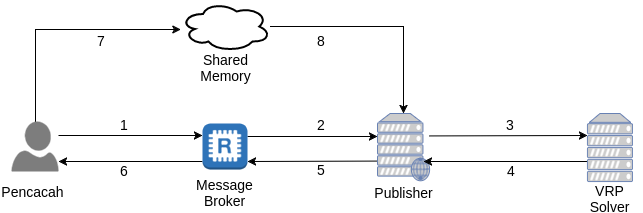
\includegraphics[width=\textwidth]{Resources/Images/component-interaction}
	\captionsetup{format=hang}
	\caption{Interaksi antar komponen dalam pengujian}
	\label{fig:component-interaction}
\end{figure}


%-----------------------------------------------------------------------------%
\subsubsection{\textit{Message Broker Setup}}
\label{ssec:broker-setup}
%-----------------------------------------------------------------------------%
Seluruh skenario dalam pengujian ini akan menggunakan Redis sebagai \textit{message broker}. Redis merupakan \textit{in-memory data structure store} yang dapat digunakan sebagai \textit{database}, \textit{cache}, dan \textit{message broker} \citep{redis_introduction_2017}. Redis mempunyai \textit{feature} Redis Cluster, sehingga dapat dengan mudah disusun menjadi \textit{distributed message broker}. Selain itu, Redis \textit{client} tersedia dalam sebagian besar bahasa pemrograman \citep{redis_clients_2017}, sehingga memungkinkan pemilihan bahasa pemrograman dalam implementasi sistem secara lebih fleksibel.


Pada penelitian ini, Redis Cluster dikonfigurasi dengan menggunakan 6 (enam) buah \textit{nodes}, 3 (tiga) node digunakan sebagai \textit{master} dan sisanya sebagai \textit{slave}. Konfigurasi Redis Cluster pada setiap node diilustrasikan pada Kode \autoref{lst:redis_conf}. Dalam konteks Redis, master dapat dianggap sebagai partisi, dan slave dianggap sebagai replikasi dari master. Seluruh node, baik master maupun slave dapat digunakan sebagai \textit{entrypoint} bagi \textit{client}.


\begin{listing}[!]
	\captionsetup{format=hang}
	\caption{Konfigurasi Redis Cluster}
	\label{lst:redis_conf}
	\begin{minted}[showspaces=false,breaklines=true]{java}
cluster-enabled yes
cluster-node-timeout 5000
cluster-config-file nodes.conf
appendonly yes
dir /data
	\end{minted}
\end{listing}


\textit{Nodes} Redis yang telah dikonfigurasi dan dijalankan, dapat digunakan untuk membuat cluster dengan memanfaatkan  \textit{script} \textbf{redis-trib.rb} yang telah disediakan oleh Redis. \textit{Command} yang digunakan dalam pembuatan cluster serta  \textit{response} yang diperoleh diilustrasikan pada Kode \autoref{lst:redis_trib_cluster} dan \autoref{lst:redis_trib_cluster_response}. \autoref{fig:test-flowchart-normal-global-broker} 
menyajikan \textit{flowchart} subsistem \textit{message broker setup}. 


\begin{listing}[!]
	\captionsetup{format=hang}
	\caption{Pembuatan Redis Cluster}
	\label{lst:redis_trib_cluster}
	\begin{minted}[showspaces=false,breaklines=true]{java}
/redis-trib.rb create --replicas 1 172.17.0.3 172.17.0.4 172.17.0.5 172.17.0.6 172.17.0.7 172.17.0.8
	\end{minted}
\end{listing}


\begin{listing}[!]
	\captionsetup{format=hang}
	\caption{Respon Pembuatan Redis Cluster}
	\label{lst:redis_trib_cluster_response}
	\begin{minted}[showspaces=false,breaklines=true]{java}
Creating cluster
Performing hash slots allocation on 6 nodes...
Using 3 masters:
172.17.0.3:6379
172.17.0.4:6379
172.17.0.5:6379
Adding replica 172.17.0.6:6379 to 172.17.0.3:6379
Adding replica 172.17.0.7:6379 to 172.17.0.4:6379
Adding replica 172.17.0.8:6379 to 172.17.0.5:6379
M: 2f0c681921fe52900a6774fb2cc808a8c4e69216 172.17.0.3:6379
slots:0-5460 (5461 slots) master
M: 41a343142847138301ceeb710206284a50bb44a0 172.17.0.4:6379
slots:5461-10922 (5462 slots) master
M: 88ae20b9e75dd5aa58973f13aa89479f52cedfd3 172.17.0.5:6379
slots:10923-16383 (5461 slots) master
S: c5f6764d82ed10793c0c81e54830b4f68b1eacd7 172.17.0.6:6379
replicates 2f0c681921fe52900a6774fb2cc808a8c4e69216
S: 5906f61963d4a5a45478736d976b79db4280b3c7 172.17.0.7:6379
replicates 41a343142847138301ceeb710206284a50bb44a0
S: 635ed817b134b5d14bffd61fe9089867037fee8c 172.17.0.8:6379
replicates 88ae20b9e75dd5aa58973f13aa89479f52cedfd3
Can I set the above configuration? (type 'yes' to accept): yes
Nodes configuration updated
Assign a different config epoch to each node
Sending CLUSTER MEET messages to join the cluster
Waiting for the cluster to join...
Performing Cluster Check (using node 172.17.0.3:6379)
M: 2f0c681921fe52900a6774fb2cc808a8c4e69216 172.17.0.3:6379
slots:0-5460 (5461 slots) master
1 additional replica(s)
M: 88ae20b9e75dd5aa58973f13aa89479f52cedfd3 172.17.0.5:6379
slots:10923-16383 (5461 slots) master
1 additional replica(s)
S: c5f6764d82ed10793c0c81e54830b4f68b1eacd7 172.17.0.6:6379
slots: (0 slots) slave
replicates 2f0c681921fe52900a6774fb2cc808a8c4e69216
M: 41a343142847138301ceeb710206284a50bb44a0 172.17.0.4:6379
slots:5461-10922 (5462 slots) master
1 additional replica(s)
S: 635ed817b134b5d14bffd61fe9089867037fee8c 172.17.0.8:6379
slots: (0 slots) slave
replicates 88ae20b9e75dd5aa58973f13aa89479f52cedfd3
S: 5906f61963d4a5a45478736d976b79db4280b3c7 172.17.0.7:6379
slots: (0 slots) slave
replicates 41a343142847138301ceeb710206284a50bb44a0
[OK] All nodes agree about slots configuration.
Check for open slots...
Check slots coverage...
[OK] All 16384 slots covered.
	\end{minted}
\end{listing}


%-----------------------------------------------------------------------------%
\subsubsection{\textit{Publisher Setup}}
%-----------------------------------------------------------------------------%
Publisher dikonfigurasi dan dijalankan pada lingkungan yang telah didefinisikan pada \autoref{ssec:test-environment}, sesuai dengan alur yang digambarkan pada \autoref{fig:test-flowchart-normal-global-publisher}. Format penggunaan Publisher diilustrasikan pada \autoref{lst:publisher-usage}.


\begin{listing}[!]
	\captionsetup{format=hang}
	\caption{Format penggunaan Publisher}
	\label{lst:publisher-usage}
	\begin{minted}[showspaces=false,breaklines=true]{bash}
Usage: mdvrp-redis-producer [options]

Run location recommendation server

Options:
-h, --help            show this help message and exit
-b BIN, --coes-bin=BIN
Binary of CoES MDVRP library
-D D, --data=D        Data problem file
-C C, --cost-file=C   Cost matrix file
-O O, --output-dir=O  Output directory
-t, --use-timestamp   Append timestamp to output directory
-B B, --broker-url=B  Redis broker URL
-X X, --solver-execution-time=X
VRP Solver execution time
	\end{minted}
\end{listing}


%-----------------------------------------------------------------------------%
\subsubsection{\textit{Subscriber Setup}}
\label{sssec:subscriber-setup}
%-----------------------------------------------------------------------------%
Pengujian memerlukan sebuah program tambahan yang berperan sebagai pencacah/\textit{subscriber}. Alur kerja dari tiap-tiap \textit{subscriber} (\autoref{fig:test-flowchart-normal-global-subscriber}) adalah sebagai berikut:


\begin{enumerate}
	\item Lakukan \textit{subscription} (pengiriman \textit{request}) pada \textit{message broker} dengan topik \textit{current location} dari \textit{subscriber}. 
	\item Sebuat \textit{reply} akan diterima dari \textit{publisher} yang dikirim melalui \textit{message broker} berupa lokasi pencacahan berikutnya yang akan dikunjungi. 
	\item Lakukan perjalanan ke lokasi yang akan dikunjungi yang disimulasikan dengan `\textit{sleep}'
	\item Setelah tiba di lokasi, simpan \textit{current location} pada \textit{shared memory} 
	\item Lakukan pencacahan yang disimulasikan dengan \textit{sleep}, 
	\item Ulangi proses dari langkah pertama.
\end{enumerate}


\begin{figure}[!]
	\centering
	\begin{subfigure}[t]{0.3\textwidth}
		\centering
		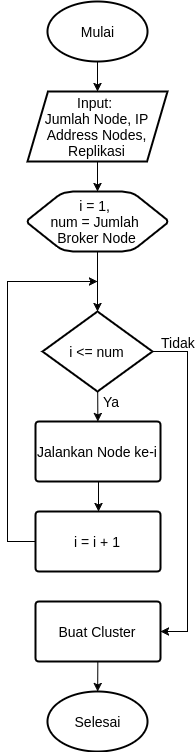
\includegraphics[width=\textwidth]{Resources/Images/test-flowchart-normal-global-broker}
		\caption{\textit{Flowchart Message Broker}}
		\label{fig:test-flowchart-normal-global-broker}
	\end{subfigure}%
	~
	\begin{subfigure}[t]{0.39\textwidth}
		\centering
		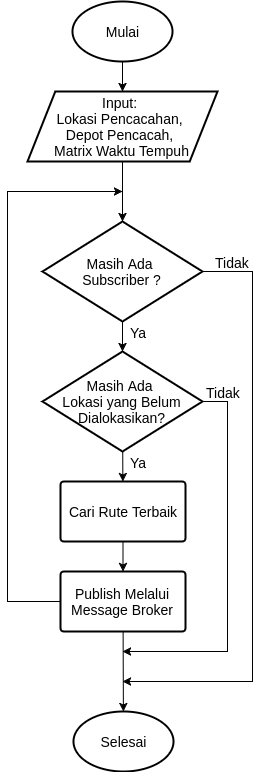
\includegraphics[width=\textwidth]{Resources/Images/test-flowchart-normal-global-publisher}
		\caption{\textit{Flowchart Publisher}}
		\label{fig:test-flowchart-normal-global-publisher}
	\end{subfigure}%
	~
	\begin{subfigure}[t]{0.31\textwidth}
		\centering
		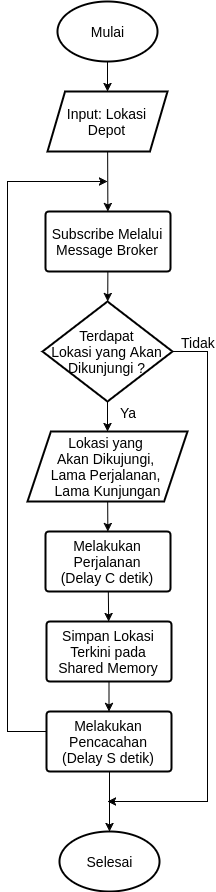
\includegraphics[width=\textwidth]{Resources/Images/test-flowchart-normal-global-subscriber}
		\caption{\textit{Flowchart Subscriber}}
		\label{fig:test-flowchart-normal-global-subscriber}
	\end{subfigure}
	\captionsetup{format=hang}
	\caption{\textit{Flowchart} Subsistem pada Pengujian}
	\label{fig:test-flowchart-normal-global}
\end{figure}


%-----------------------------------------------------------------------------%
\subsubsection{Pengujian Kondisi Normal dengan \textit{Service Time} pada Data Cordeau}
\label{ssec:test-normal-service-time-cordeau}
%-----------------------------------------------------------------------------%
Skenario pengujian kondisi normal dimaksudkan untuk membandingkan sistem yang dijalankan pada kondisi normal dan tidak ada sesuatupun yang menyebabkan penundaaan. Pengujian kondisi ini dilakukan untuk tiap-tiap \textit{instance} Cordeau. \textit{Instance} Cordeau dianggap dapat digunakan dengan beberapa penyesuaian istilah, yaitu pelanggan dianalogikan dengan wilayah kerja dan kendaraan dianalogikan dengan pencacah. \textit{Instance} Cordeau yang digunakan dalam pengujian adalah \textit{instance} P01 sampai P07, karena masing-masing \textit{instance} mewakili kondisi acak, baik dari segi jumlah pelanggan, jumlah kendaraan, serta koordinat pelanggan dan depot kendaraan.


\textit{Instance} Cordeau tipe 2 tidak menyertakan lama waktu pencacahan pada tiap-tiap pelanggan. Agar mencerminkan kondisi pencacahan yang sebenarnya, data lama waktu pencacahan akan dibuat secara acak dengan mengikuti komposisi dari \citep{sudman_time_1965}, yaitu:
\begin{enumerate}
	\item 21 persen dari total waktu digunakan untuk perpindahan antar wilayah kerja, 
	\item 15 persen dari total waktu digunakan untuk perpindahan antar rumah tangga dalam wilayah kerja, 
	\item 37 persen dari total waktu digunakan untuk wawancara seluruh rumah tangga, dan 
	\item 27 persen untuk hal-hal yang lain, seperti pengenalan wilayah dan perbaikan data.
\end{enumerate}
Lama waktu pencacahan merupakan gabungan dari keseluruhan waktu perpindahan antar rumah tangga dan waktu wawancara. Meskipun komposisi waktu \citep{sudman_time_1965} dinilai tidak relevan lagi, tetapi dari segi komponen yang menyusun waktu pencacahan dinilai masih cukup relevan. Dengan demikian, komposisi dari tiap-tiap \textit{instance} Cordeau yang digunakan dalam pengujian adalah sebagai berikut:
\begin{enumerate}
	\item Instance P01 terdiri dari 50 pelanggan dan 5 kendaraan, lama wawancara pada tiap-tiap rumah tangga 27.58 menit dengan standar deviasi 12.13 menit.
	\item Instance P02 terdiri dari 50 pelanggan dan 4 kendaraan, lama wawancara pada tiap-tiap rumah tangga 27.58 menit dengan standar deviasi 12.13 menit.
	\item Instance P03 terdiri dari 75 pelanggan dan 5 kendaraan, lama wawancara pada tiap-tiap rumah tangga 27.58 menit dengan standar deviasi 12.13 menit.
	\item Instance P04 terdiri dari 100 pelanggan dan 2 kendaraan, lama wawancara pada tiap-tiap rumah tangga 27.58 menit dengan standar deviasi 12.13 menit.
	\item Instance P05 terdiri dari 100 pelanggan dan 2 kendaraan, lama wawancara pada tiap-tiap rumah tangga 27.58 menit dengan standar deviasi 12.13 menit.
	\item Instance P06 terdiri dari 100 pelanggan dan 3 kendaraan, lama wawancara pada tiap-tiap rumah tangga 27.58 menit dengan standar deviasi 12.13 menit.
	\item Instance P07 terdiri dari 100 pelanggan dan 4 kendaraan, lama wawancara pada tiap-tiap rumah tangga 27.58 menit dengan standar deviasi 12.13 menit.
\end{enumerate}


Setiap \textit{instance} data diuji sebanyak 100 (seratus) kali untuk membuktikan bahwa hasil yang diperoleh konsisten. Pada tiap-tiap pengujian akan diperoleh rute untuk setiap petugas pencacahan seperti contoh berikut:
\begin{itemize}
	\item \textit{Vehicle} A = Loc1 $\rightarrow$ Loc5 $\rightarrow$ Loc15 $\rightarrow$ Loc12
	\item \textit{Vehicle} B = Loc 6 $\rightarrow$ Loc2 $\rightarrow$ Loc16 $\rightarrow$ Loc3
	\item \textit{Vehicle} C = Loc4 $\rightarrow$ Loc8 $\rightarrow$ Loc14 $\rightarrow$ Loc 7
	\item \textit{Vehicle} D = Loc9 $\rightarrow$ Loc10 $\rightarrow$ Loc11 $\rightarrow$ Loc12
\end{itemize}
Waktu total untuk tiap-tiap rute dihitung dengan melakukan penjumlahan waktu tempuh dan waktu pencacahan dari seluruh lokasi yang dikunjungi pada rute tersebut. Selain itu, standar deviasi dari waktu total untuk tiap-tiap rute juga dihitung untuk menggambarkan kesenjangan waktu penyelesaian pencacahan.


\begin{longtable}[!]{c|cccc}
	\captionsetup{format=hang}
	\caption{Rata-rata Lama Pencacahan Masing-masing Petugas (Hari) Dari 100 Pengujian Kondisi Normal dengan Waktu Pencacahan pada Data Cordeau}
	\label{tbl:test_result_cordeau_tw_mean_of_total_time}\\
	\toprule
	& \multicolumn{2}{c}{MDVRP berbasis CoEAs} & \multicolumn{2}{c}{MDVRP berbasis CoEAs dan Pub/Sub}
	\tabularnewline
	\textit{\textit{Instance}} & \MyHead{2cm}{Rata-rata} & \MyHead{2cm}{Std. Error} & \MyHead{2cm}{Rata-rata} & \MyHead{2cm}{Std. Error} \\ 
	\midrule
	\endfirsthead
	\toprule
	\textit{\textit{Instance}} & \MyHead{2cm}{Rata-rata} & \MyHead{2cm}{Std. Error} & \MyHead{2cm}{Rata-rata} & \MyHead{2cm}{Std. Error} \\ 
	\midrule
	\endhead
	\bottomrule
	\endfoot
	d01 & 13  & 0 & 13  & 0,05 \\
	d02  & 13 & 0 & 13 & 0,05 \\
	d03  & 16 & 0 & 16 & 0,00 \\
	d04  & 51 & 0 & 51 & 0,05 \\
	d05 & 51 & 0 & 51 & 0,00 \\
	d06  & 34 & 0 & 34 & 0,00 \\
	d07  & 36  & 0 & 36 & 0,00 \\
\end{longtable}


\begin{figure}[!]
	\centering
	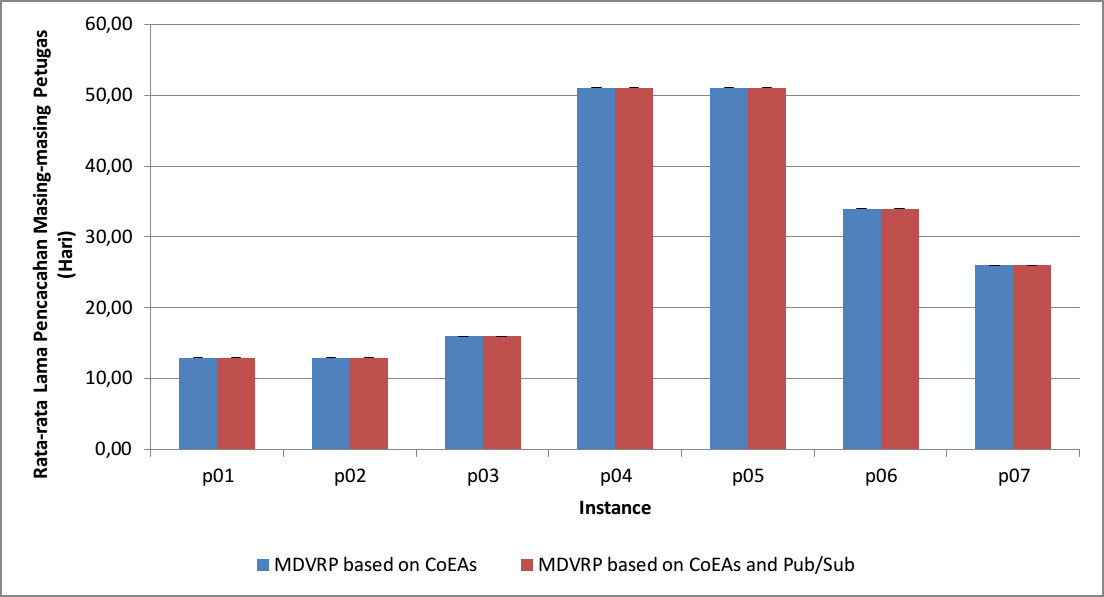
\includegraphics[width=\textwidth]{Resources/Images/test_result_cordeau_tw_mean_of_total_time}
	\captionsetup{format=hang}
	\caption{Rata-rata Lama Pencacahan Masing-masing Petugas (Hari) Dari 100 Pengujian Kondisi Normal dengan Waktu Pencacahan pada Data Cordeau}
	\label{fig:test_result_cordeau_tw_mean_of_total_time}
\end{figure}


\begin{longtable}[!]{c|cccc}
	\captionsetup{format=hang}
	\caption{Standar Deviasi Lama Pencacahan Masing-masing Petugas (Hari) Dari 100 Pengujian Kondisi Normal dengan Waktu Pencacahan pada Data Cordeau}
	\label{tbl:test_result_cordeau_tw_stdev_of_total_time}\\
	\toprule
	& \multicolumn{2}{c}{MDVRP berbasis CoEAs} & \multicolumn{2}{c}{MDVRP berbasis CoEAs dan Pub/Sub}
	\tabularnewline
	\textit{\textit{Instance}} & \MyHead{2cm}{Std. Deviasi} & \MyHead{2cm}{Std. Error} & \MyHead{2cm}{Std. Deviasi} & \MyHead{2cm}{Std. Error} \\ 
	\midrule
	\endfirsthead
	\toprule
	\textit{\textit{Instance}} & \MyHead{2cm}{Std. Deviasi} & \MyHead{2cm}{Std. Error} & \MyHead{2cm}{Std. Deviasi} & \MyHead{2cm}{Std. Error} \\ 
	\midrule
	\endhead
	\bottomrule
	\endfoot
	d01 & 2  & 0 & 1,02 & 0,04 \\
	d02  & 2 & 0 & 1,11 & 0,05 \\
	d03  & 5  & 0 & 1,80 & 0,09 \\
	d04  & 7 & 0 & 2,39 & 0,30 \\
	d05 & 9  & 0 & 5,13 & 0,58 \\
	d06  & 7 & 0 & 3,62 & 0,34 \\
	d07  & 6  & 0 & 2,93 & 0,20 \\
\end{longtable}


\begin{figure}[!]
	\centering
	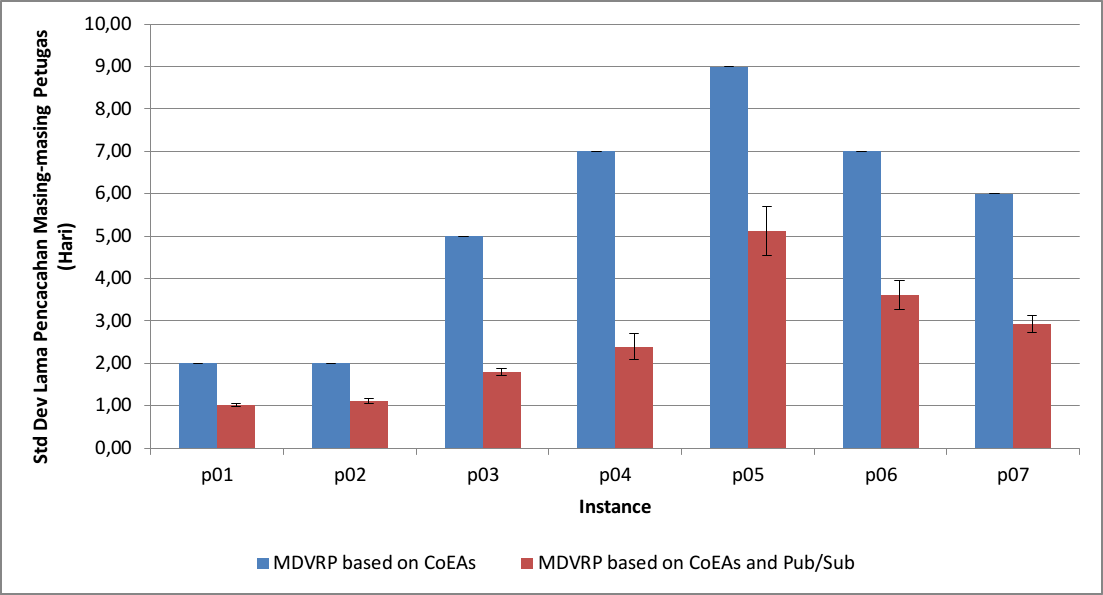
\includegraphics[width=\textwidth]{Resources/Images/test_result_cordeau_tw_stdev_of_total_time}
	\captionsetup{format=hang}
	\caption{Standar Deviasi Lama Pencacahan Masing-masing Petugas (Hari) Dari 100 Pengujian Kondisi Normal dengan Waktu Pencacahan pada Data Cordeau}
	\label{fig:test_result_cordeau_tw_stdev_of_total_time}
\end{figure}


Berdasarkan hasil pengujian terhadap 7 (tujuh) buah \textit{instance} yang tiap-tiap \textit{instance} dijalankan sebanyak 100 kali, diperoleh hasil bahwa dengan menggunakan sistem usulan maupun program pembanding menghasilkan rata-rata yang sama untuk jumlah hari pencacahan setiap pencacah, seperti digambarkan pada \autoref{fig:test_result_cordeau_tw_mean_of_total_time}. Akan tetapi, dari segi variasi hari pencacahan untuk setiap petugas, diperoleh hasil bahwa sistem usulan menghasilkan standar deviasi yang lebih rendah untuk seluruh instance dibandingkan dengan program pembanding, seperti digambarkan pada \autoref{fig:test_result_cordeau_tw_stdev_of_total_time}. Hal ini menunjukkan bahwa sistem usulan, yaitu MDVRP berbasis CoEAs dan mekansime \textit{publish/subscribe}, lebih efisien jika dibandingkan dengan program pembanding, yaitu MDVRP berbasis CoEAs dan mekansime \textit{publish/subscribe}, karena menghasilkan rute dengan beban tugas yang lebih merata. Hal ini berdampak positif kepada total waktu seluruh kegiatan yang dengan sistem usulan menjadi lebih pendek dibandingkan sistem pembanding, seperti digambarkan pada \autoref{fig:test_result_cordeau_tw_mean_stdev_of_total_time}.


\begin{figure}[!]
	\centering
	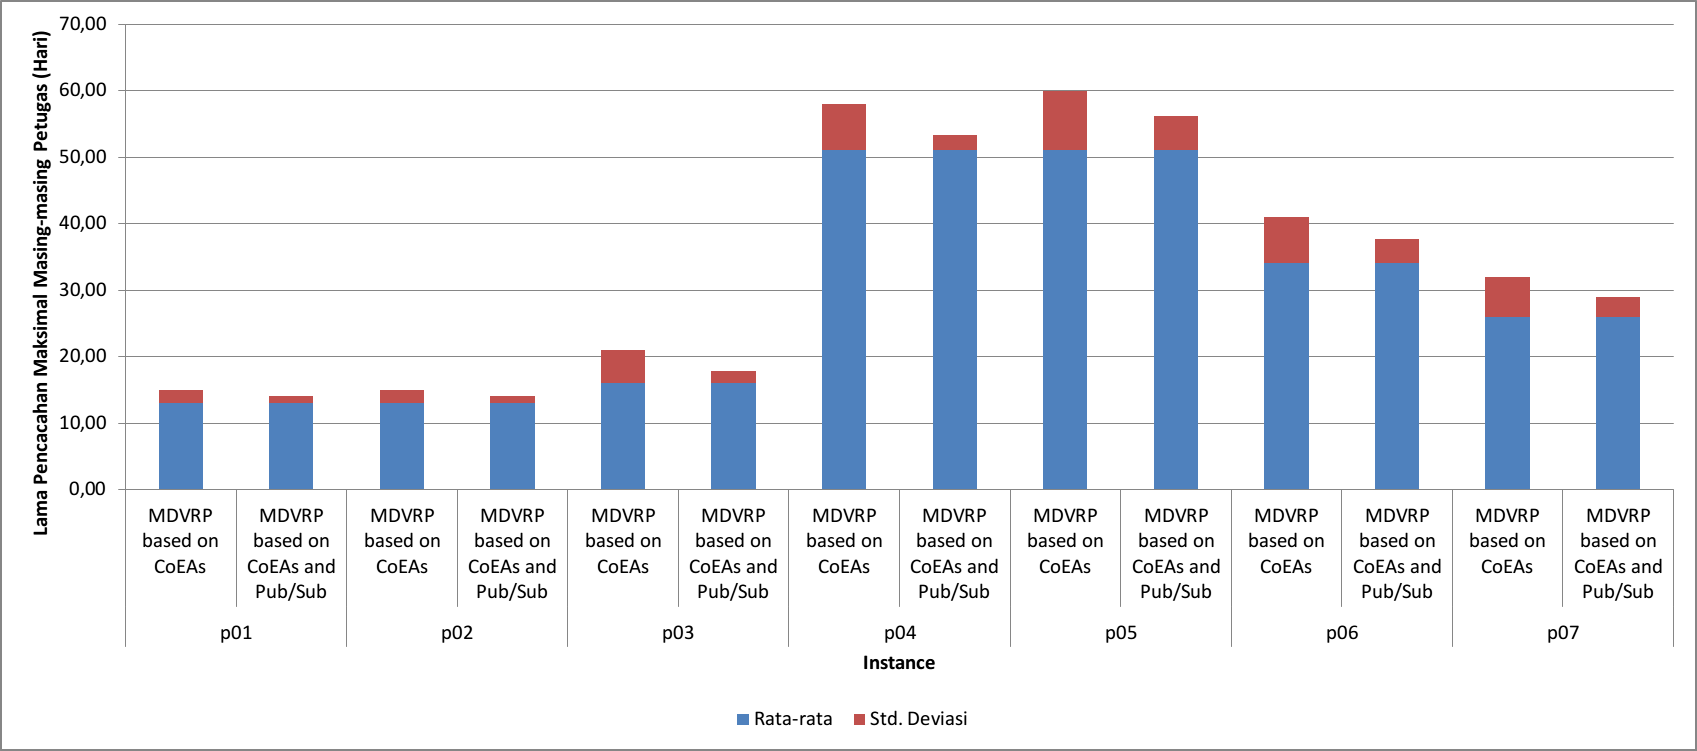
\includegraphics[width=\textwidth]{Resources/Images/test_result_cordeau_tw_mean_stdev_of_total_time}
	\captionsetup{format=hang}
	\caption{Maksimum Lama Pencacahan Masing-masing Petugas (Hari) Dari 100 Pengujian Kondisi Normal dengan Waktu Pencacahan pada Data Cordeau}
	\label{fig:test_result_cordeau_tw_mean_stdev_of_total_time}
\end{figure}


%-----------------------------------------------------------------------------%
\subsubsection{Pengujian Kondisi Normal dengan \textit{Service Time} pada Data Lapangan}
\label{ssec:test-normal-service-time-field}
%-----------------------------------------------------------------------------%
Skenario pengujian kondisi ini memiliki tujuan yang sama dengan pengujian dengan \textit{instance} Cordeau pada \autoref{ssec:test-normal-service-time-cordeau}, tetapi data lokasi yang digunakan adalah lokasi yang sebenarnya. Perbedaan lainnya adalah pada pengujian ini koordinat lokasi yang digunakan pada tiap-tiap instance sama, tetapi lama wawancara yang digunakan berbeda-beda. Sementara itu, data lama waktu pencacahan juga akan dibuat secara acak dengan mengikuti komposisi dari \citep{sudman_time_1965}. Dengan demikian, data lapangan yang digunakan memiliki komposisi sebagai berikut:
\begin{enumerate}
	\item \textit{Instance} TW1 terdiri dari 182 pelanggan dan 15 kendaraan, lama wawancara pada tiap-tiap rumah tangga 27.58 menit dengan standar deviasi 4,13 menit.
	\item \textit{Instance} TW2 terdiri dari 182 pelanggan dan 15 kendaraan, lama wawancara pada tiap-tiap rumah tangga 71.58 menit dengan standar deviasi 12.16 menit.
	\item \textit{Instance} TW3 terdiri dari 182 pelanggan dan 15 kendaraan, lama wawancara pada tiap-tiap rumah tangga 27.35 menit dengan standar deviasi 25.34 menit.
	\item \textit{Instance} TW4 terdiri dari 182 pelanggan dan 15 kendaraan, lama wawancara pada tiap-tiap rumah tangga 71.58 menit dengan standar deviasi 56.87 menit.
\end{enumerate}


Setiap \textit{instance} data diuji sebanyak 100 (seratus) kali untuk membuktikan bahwa hasil yang diperoleh konsisten. Pada tiap-tiap pengujian akan diperoleh rute untuk setiap petugas pencacahan seperti contoh berikut:
\begin{itemize}
	\item \textit{Vehicle} A = Loc1 $\rightarrow$ Loc5 $\rightarrow$ Loc15 $\rightarrow$ Loc12
	\item \textit{Vehicle} B = Loc 6 $\rightarrow$ Loc2 $\rightarrow$ Loc16 $\rightarrow$ Loc3
	\item \textit{Vehicle} C = Loc4 $\rightarrow$ Loc8 $\rightarrow$ Loc14 $\rightarrow$ Loc 7
	\item \textit{Vehicle} D = Loc9 $\rightarrow$ Loc10 $\rightarrow$ Loc11 $\rightarrow$ Loc12
\end{itemize}
Waktu total untuk tiap-tiap rute dihitung dengan melakukan penjumlahan waktu tempuh dan waktu pencacahan dari seluruh lokasi yang dikunjungi pada rute tersebut. Selain itu, standar deviasi dari waktu total untuk tiap-tiap rute juga dihitung untuk menggambarkan kesenjangan waktu penyelesaian pencacahan


\begin{longtable}[!]{c|cccc}
	\captionsetup{format=hang}
	\caption{Rata-rata Lama Pencacahan Masing-masing Petugas (Hari) Dari 100 Pengujian Kondisi Normal dengan Waktu Pencacahan pada Data Lapangan}
	\label{tbl:test_result_real_tw_mean_of_total_time}\\
	\toprule
	& \multicolumn{2}{c}{MDVRP berbasis CoEAs} & \multicolumn{2}{c}{MDVRP berbasis CoEAs dan Pub/Sub}
	\tabularnewline
	\textit{\textit{Instance}} & \MyHead{2cm}{Rata-rata} & \MyHead{2cm}{Std. Error} & \MyHead{2cm}{Rata-rata} & \MyHead{2cm}{Std. Error} \\ 
	\midrule
	\endfirsthead
	\toprule
	\textit{\textit{Instance}} & \MyHead{2cm}{Rata-rata} & \MyHead{2cm}{Std. Error} & \MyHead{2cm}{Rata-rata} & \MyHead{2cm}{Std. Error} \\ 
	\midrule
	\endhead
	\bottomrule
	\endfoot
	tw01 & 13  & 0 & 13  & 0 \\
	tw02  & 13 & 0 & 13  & 0 \\
	tw03  & 13  & 0 & 13  & 0 \\
	tw04  & 13 & 0 & 13  & 0 \\
\end{longtable}


\begin{figure}[!]
	\centering
	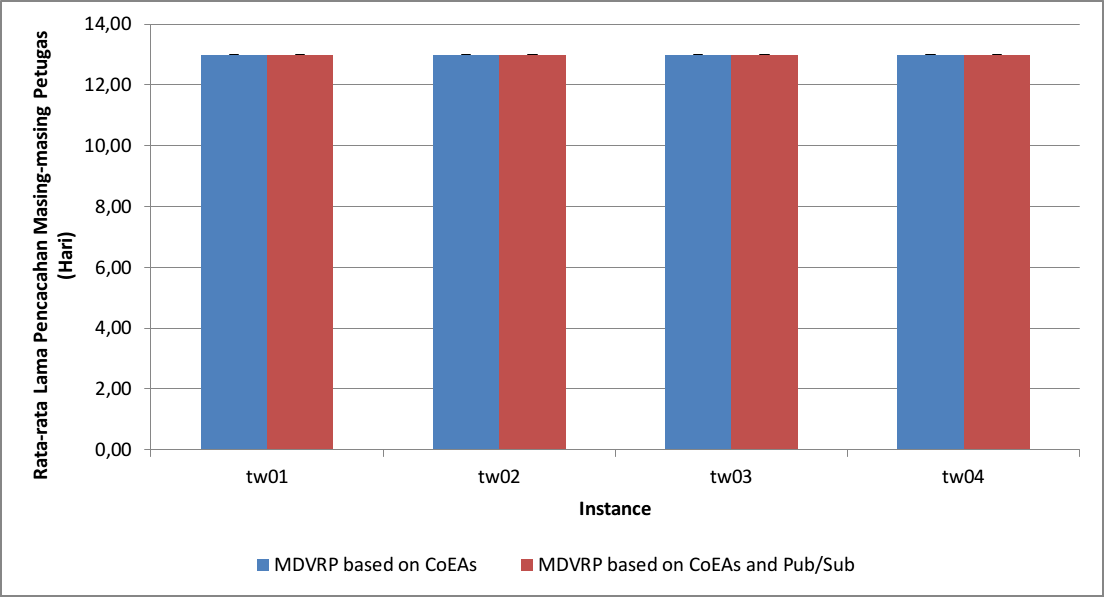
\includegraphics[width=\textwidth]{Resources/Images/test_result_real_tw_mean_of_total_time}
	\captionsetup{format=hang}
	\caption{Rata-rata Lama Pencacahan Masing-masing Petugas (Hari) Dari 100 Pengujian Kondisi Normal dengan Waktu Pencacahan pada Data Lapangan}
	\label{fig:test_result_real_tw_mean_of_total_time}
\end{figure}


\begin{longtable}[!]{c|cccc}
	\captionsetup{format=hang}
	\caption{Standar Deviasi Lama Pencacahan Masing-masing Petugas (Hari) Dari 100 Pengujian Kondisi Normal dengan Waktu Pencacahan pada Data Lapangan}
	\label{tbl:test_result_real_tw_stdev_of_total_time}\\
	\toprule
	& \multicolumn{2}{c}{MDVRP berbasis CoEAs} & \multicolumn{2}{c}{MDVRP berbasis CoEAs dan Pub/Sub}
	\tabularnewline
	\textit{\textit{Instance}} & \MyHead{2cm}{Std. Deviasi} & \MyHead{2cm}{Std. Error} & \MyHead{2cm}{Std. Deviasi} & \MyHead{2cm}{Std. Error} \\ 
	\midrule
	\endfirsthead
	\toprule
	\textit{\textit{Instance}} & \MyHead{2cm}{Std. Deviasi} & \MyHead{2cm}{Std. Error} & \MyHead{2cm}{Std. Deviasi} & \MyHead{2cm}{Std. Error} \\ 
	\midrule
	\endhead
	\bottomrule
	\endfoot
	tw01 & 4  & 0 & 1,56 & 0,06 \\
	tw02  & 4 & 0 & 0,08 & 0,03 \\
	tw03  & 4  & 0 & 0,83 & 0,04 \\
	tw04  & 4 & 0 & 0,04 & 0,02 \\
\end{longtable}


\begin{figure}[!]
	\centering
	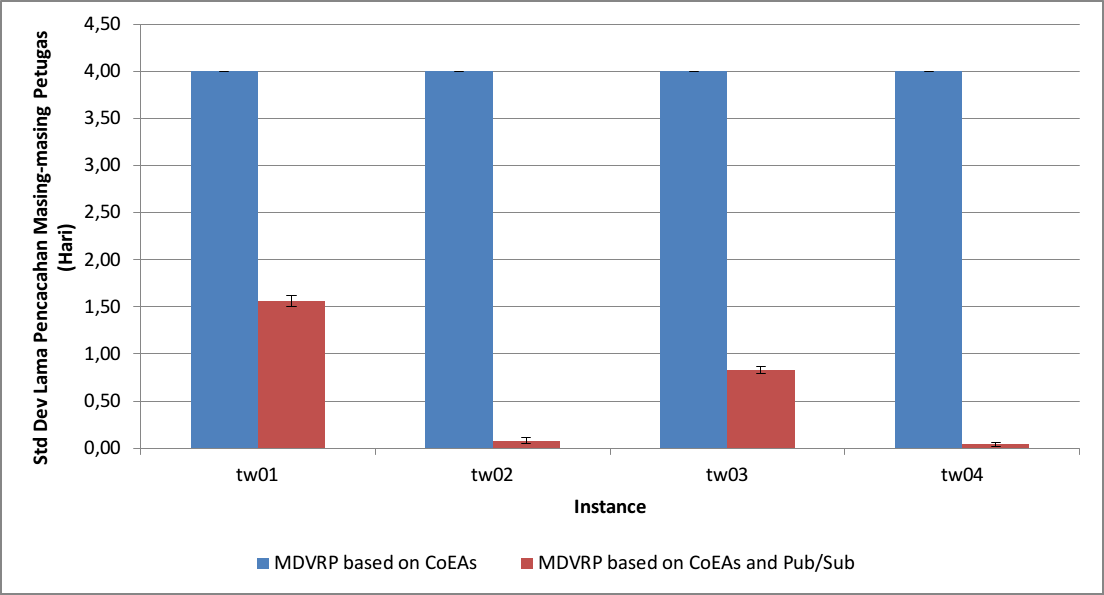
\includegraphics[width=\textwidth]{Resources/Images/test_result_real_tw_stdev_of_total_time}
	\captionsetup{format=hang}
	\caption{Standar Deviasi Lama Pencacahan Masing-masing Petugas (Hari) Dari 100 Pengujian Kondisi Normal dengan Waktu Pencacahan pada Data Lapangan}
	\label{fig:test_result_real_tw_stdev_of_total_time}
\end{figure}


\begin{figure}[!]
	\centering
	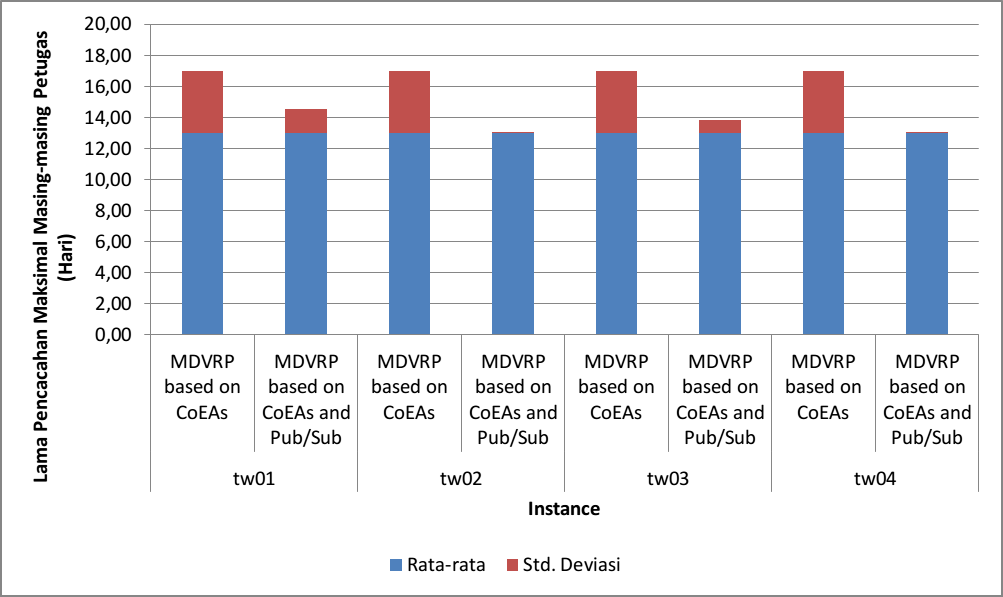
\includegraphics[width=\textwidth]{Resources/Images/test_result_real_tw_mean_stdev_of_total_time}
	\captionsetup{format=hang}
	\caption{Maksimum Lama Pencacahan Masing-masing Petugas (Hari) Dari 100 Pengujian Kondisi Normal dengan Waktu Pencacahan pada Data Lapangan}
	\label{fig:test_result_real_tw_mean_stdev_of_total_time}
\end{figure}


Berdasarkan hasil pengujian terhadap 4 (empat) buah \textit{instance} yang tiap-tiap \textit{instance} dijalankan sebanyak 100 kali, diperoleh hasil bahwa dengan menggunakan sistem usulan maupun program pembanding menghasilkan rata-rata yang sama untuk jumlah hari pencacahan setiap pencacah, seperti digambarkan pada \autoref{fig:test_result_real_tw_mean_of_total_time}. Akan tetapi, dari segi variasi hari pencacahan untuk setiap petugas, diperoleh hasil bahwa sistem usulan menghasilkan standar deviasi yang lebih rendah untuk seluruh instance dibandingkan dengan program pembanding, seperti digambarkan pada \autoref{fig:test_result_real_tw_stdev_of_total_time}. Hal ini menunjukkan bahwa sistem usulan, yaitu MDVRP berbasis CoEAs dan mekansime \textit{publish/subscribe}, lebih efisien jika dibandingkan dengan program pembanding, yaitu MDVRP berbasis CoEAs dan mekansime \textit{publish/subscribe}, karena menghasilkan rute dengan beban tugas yang lebih merata. Hal ini berdampak positif kepada total waktu seluruh kegiatan yang dengan sistem usulan menjadi lebih pendek dibandingkan sistem pembanding, seperti digambarkan pada \autoref{fig:test_result_real_tw_mean_stdev_of_total_time}.


%-----------------------------------------------------------------------------%
\subsubsection{Pengujian Kondisi \textit{Delay} dengan \textit{Service Time} pada Data Lapangan}
\label{sssec:test-delay-service-time}
%-----------------------------------------------------------------------------%
Skenario pengujian kondisi \textit{delay} dimaksudkan untuk membandingkan program yang dijalankan pada kondisi terjadi hal-hal yang menghambat jalannya pencacahan. Pengujian ini digunakan sebagai cerminan kodisi lapangan di mana pada beberapa lokasi tidak terdapat koneksi yang stabil, sehingga untuk melakukan \textit{subscription} lokasi berikutnya perlu berpindah ke lokasi lain. Pengujian dilakukan sebanyak 7 (tujuh) kali yang pada tiap-tiap pengujian mencerminkan kondisi yang berbeda, yaitu:

\begin{enumerate}
	\item Pengujian dengan kode \textit{instance} d01 menggambarkan kondisi normal. Parameter yang digunakan pada \textit{instance} ini adalah sebagai berikut:
	\begin{itemize}
		\item Jumlah responden pada setiap segmen/blok sensus adalah 10 rumah tangga
		\item Rata-rata wawancara pada setiap rumah tangga 27,58 menit dengan standar deviasi 12,13 menit.
		\item Rata-rata waktu yang diperlukan untuk mendapatkan koneksi internet sebesar 5 menit dengan standar deviasi 3 menit.
	\end{itemize}
	\item Pengujian dengan kode \textit{instance} d02 menggambarkan kondisi pencacahan dengan anggota rumah tangga sedikit dan relatif homogen, dengan koneksi internet relatif mudah didapatkan. Parameter yang digunakan pada \textit{instance} ini adalah sebagai berikut:
	\begin{itemize}
		\item Jumlah responden pada setiap segmen/blok sensus adalah 10 rumah tangga
		\item Rata-rata wawancara pada setiap rumah tangga 27,58 menit dengan standar deviasi 4,16 menit.
		\item Rata-rata waktu yang diperlukan untuk mendapatkan koneksi internet sebesar 5 menit dengan standar deviasi 3 menit.
	\end{itemize}
	\item Pengujian dengan kode \textit{instance} d03 menggambarkan kondisi pencacahan dengan anggota rumah tangga sedikit dan relatif homogen, dengan koneksi internet secara umum sulit didapatkan. Parameter yang digunakan pada \textit{instance} ini adalah sebagai berikut:
	\begin{itemize}
		\item Jumlah responden pada setiap segmen/blok sensus adalah 10 rumah tangga
		\item Rata-rata wawancara pada setiap rumah tangga 27,58 menit dengan standar deviasi 4,16 menit.
		\item Rata-rata waktu yang diperlukan untuk mendapatkan koneksi internet sebesar 60 menit dengan standar deviasi 3 menit.
	\end{itemize}
	\item Pengujian dengan kode \textit{instance} d04 menggambarkan kondisi pencacahan dengan anggota rumah tangga banyak dan relatif homogen, dengan koneksi internet relatif mudah didapatkan. Parameter yang digunakan pada \textit{instance} ini adalah sebagai berikut:
	\begin{itemize}
		\item Jumlah responden pada setiap segmen/blok sensus adalah 10 rumah tangga
		\item Rata-rata wawancara pada setiap rumah tangga 71,58 menit dengan standar deviasi 12,16 menit.
		\item Rata-rata waktu yang diperlukan untuk mendapatkan koneksi internet sebesar 5 menit dengan standar deviasi 3 menit.
	\end{itemize}
	\item Pengujian dengan kode \textit{instance} d05 menggambarkan kondisi pencacahan dengan anggota rumah tangga banyak dan relatif homogen, dengan koneksi internet secara umum sulit didapatkan. Parameter yang digunakan pada \textit{instance} ini adalah sebagai berikut:
	\begin{itemize}
		\item Jumlah responden pada setiap segmen/blok sensus adalah 10 rumah tangga
		\item Rata-rata wawancara pada setiap rumah tangga 71,58 menit dengan standar deviasi 12,16 menit.
		\item Rata-rata waktu yang diperlukan untuk mendapatkan koneksi internet sebesar 60 menit dengan standar deviasi 3 menit.
	\end{itemize}
	\item Pengujian dengan kode \textit{instance} d06 menggambarkan kondisi pencacahan dengan rata-rata anggota rumah tangga sedikit tetapi memiliki variasi tinggi, dengan koneksi internet secara umum sulit didapatkan. Parameter yang digunakan pada \textit{instance} ini adalah sebagai berikut:
	\begin{itemize}
		\item Jumlah responden pada setiap segmen/blok sensus adalah 10 rumah tangga
		\item Rata-rata wawancara pada setiap rumah tangga 27,58 menit dengan standar deviasi 25,16 menit.
		\item Rata-rata waktu yang diperlukan untuk mendapatkan koneksi internet sebesar 60 menit dengan standar deviasi 3 menit.
	\end{itemize}
	\item Pengujian dengan kode \textit{instance} d07 menggambarkan kondisi pencacahan dengan jarak antar rumah tangga jauh, rata-rata anggota rumah tangga banyak dan memiliki variasi tinggi, dan koneksi internet secara umum sulit didapatkan. Parameter yang digunakan pada \textit{instance} ini adalah sebagai berikut:
	\begin{itemize}
		\item Jumlah responden pada setiap segmen/blok sensus adalah 10 rumah tangga
		\item Rata-rata wawancara pada setiap rumah tangga 71,58 menit dengan standar deviasi 25,65 menit.
		\item Rata-rata waktu tempuh antar rumah tangga 30,45 menit dengan standar deviasi 22,12 menit.
		\item Rata-rata waktu yang diperlukan untuk mendapatkan koneksi internet sebesar 60 menit dengan standar deviasi 3 menit.
	\end{itemize}
\end{enumerate}


Sama dengan pengujian sebelumnya, pada pengujian ini setiap \textit{instance} data diuji sebanyak 100 (seratus) kali untuk membuktikan bahwa hasil yang diperoleh konsisten. Pada tiap-tiap pengujian akan diperoleh rute untuk setiap petugas pencacahan seperti contoh berikut:
\begin{itemize}
	\item \textit{Vehicle} A = Loc1 $\rightarrow$ Loc5 $\rightarrow$ Loc15 $\rightarrow$ Loc12
	\item \textit{Vehicle} B = Loc 6 $\rightarrow$ Loc2 $\rightarrow$ Loc16 $\rightarrow$ Loc3
	\item \textit{Vehicle} C = Loc4 $\rightarrow$ Loc8 $\rightarrow$ Loc14 $\rightarrow$ Loc 7
	\item \textit{Vehicle} D = Loc9 $\rightarrow$ Loc10 $\rightarrow$ Loc11 $\rightarrow$ Loc12
\end{itemize}
Waktu total untuk tiap-tiap rute dihitung dengan melakukan penjumlahan waktu tempuh dan waktu pencacahan dari seluruh lokasi yang dikunjungi pada rute tersebut. Selain itu, standar deviasi dari waktu total untuk tiap-tiap rute juga dihitung untuk menggambarkan kesenjangan waktu penyelesaian pencacahan.


\begin{longtable}[!]{c|cccc}
	\captionsetup{format=hang}
	\caption{Rata-rata Lama Pencacahan Masing-masing Petugas (Hari) Dari 100 Pengujian Kondisi Delay dengan Waktu Pencacahan pada Data Lapangan}
	\label{tbl:test_result_delay_real_tw_mean_of_total_time}\\
	\toprule
	& \multicolumn{2}{c}{MDVRP berbasis CoEAs} & \multicolumn{2}{c}{MDVRP berbasis CoEAs dan Pub/Sub}
	\tabularnewline
	\textit{\textit{Instance}} & \MyHead{2cm}{Rata-rata} & \MyHead{2cm}{Std. Error} & \MyHead{2cm}{Rata-rata} & \MyHead{2cm}{Std. Error} \\ 
	\midrule
	\endfirsthead
	\toprule
	\textit{\textit{Instance}} & \MyHead{2cm}{Rata-rata} & \MyHead{2cm}{Std. Error} & \MyHead{2cm}{Rata-rata} & \MyHead{2cm}{Std. Error} \\ 
	\midrule
	\endhead
	\bottomrule
	\endfoot
	d01 & 13  & 0 & 14,39  & 0,05 \\
	d02  & 13 & 0 & 14,41 & 0,05 \\
	d03  & 13  & 0 & 24,00 & 0,00 \\
	d04  & 13 & 0 & 14,38 & 0,05 \\
	d05 & 13  & 0 & 24,00 & 0,00 \\
	d06  & 13 & 0 & 24,00 & 0,00 \\
	d07  & 13  & 0 & 24,00 & 0,00 \\
\end{longtable}


\begin{figure}[!]
	\centering
	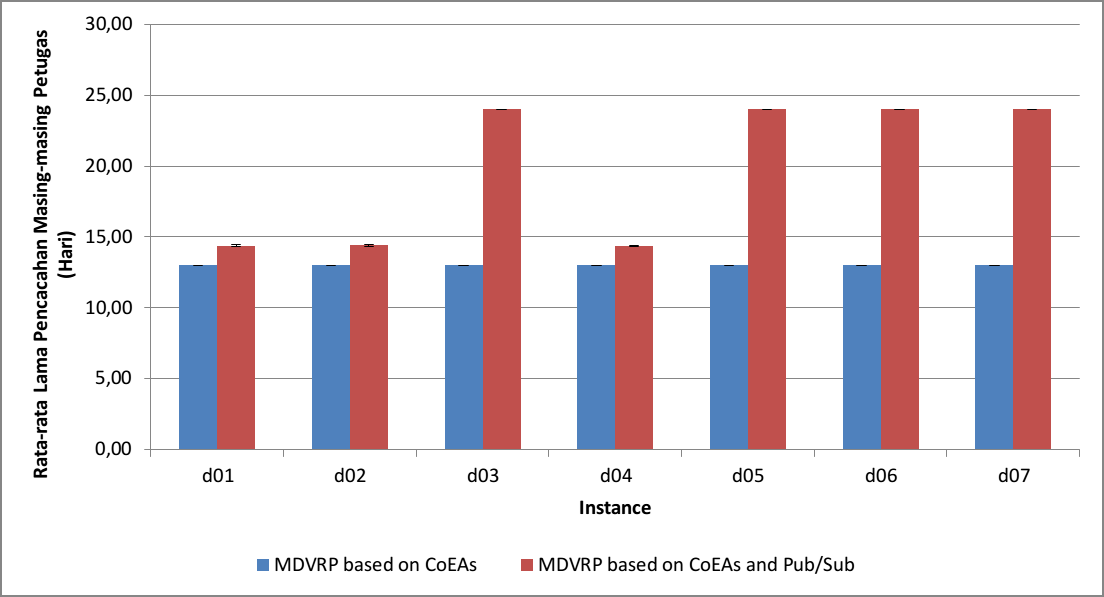
\includegraphics[width=\textwidth]{Resources/Images/test_result_delay_real_tw_mean_of_total_time}
	\captionsetup{format=hang}
	\caption{Rata-rata Lama Pencacahan Masing-masing Petugas (Hari) Dari 100 Pengujian Kondisi Normal dengan Waktu Pencacahan pada Data Lapangan}
	\label{fig:test_result_delay_real_tw_mean_of_total_time}
\end{figure}


\begin{longtable}[!]{c|cccc}
	\captionsetup{format=hang}
	\caption{Standar Deviasi Lama Pencacahan Masing-masing Petugas (Hari) Dari 100 Pengujian Kondisi Delay dengan Waktu Pencacahan pada Data Lapangan}
	\label{tbl:test_result_delay_real_tw_stdev_of_total_time}\\
	\toprule
	& \multicolumn{2}{c}{MDVRP berbasis CoEAs} & \multicolumn{2}{c}{MDVRP berbasis CoEAs dan Pub/Sub}
	\tabularnewline
	\textit{\textit{Instance}} & \MyHead{2cm}{Std. Deviasi} & \MyHead{2cm}{Std. Error} & \MyHead{2cm}{Std. Deviasi} & \MyHead{2cm}{Std. Error} \\ 
	\midrule
	\endfirsthead
	\toprule
	\textit{\textit{Instance}} & \MyHead{2cm}{Std. Deviasi} & \MyHead{2cm}{Std. Error} & \MyHead{2cm}{Std. Deviasi} & \MyHead{2cm}{Std. Error} \\ 
	\midrule
	\endhead
	\bottomrule
	\endfoot
	d01 & 4  & 0 & 1,11 & 0,04 \\
	d02  & 4 & 0 & 1,25 & 0,07 \\
	d03  & 4  & 0 & 1,15 & 0,06 \\
	d04  & 4 & 0 & 1,14 & 0,04 \\
	d05 & 4  & 0 & 1,14 & 0,05 \\
	d06  & 4 & 0 & 1,47 & 0,06 \\
	d07  & 4  & 0 & 1,20 & 0,06 \\
\end{longtable}


\begin{figure}[!]
	\centering
	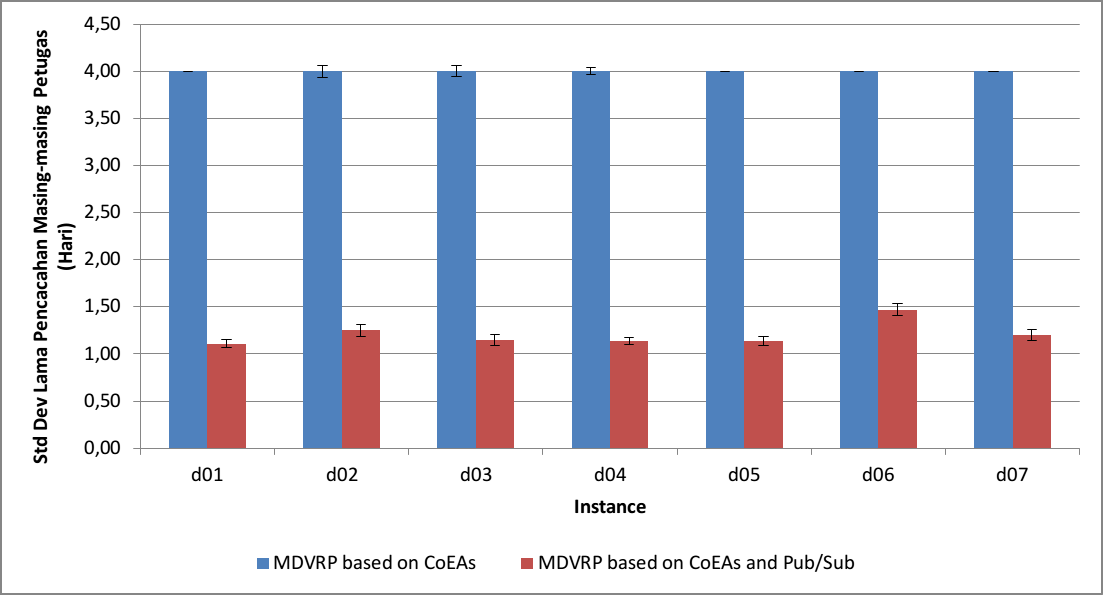
\includegraphics[width=\textwidth]{Resources/Images/test_result_delay_real_tw_stdev_of_total_time}
	\captionsetup{format=hang}
	\caption{Standar Deviasi Lama Pencacahan Masing-masing Petugas (Hari) Dari 100 Pengujian Kondisi Normal dengan Waktu Pencacahan pada Data Lapangan}
	\label{fig:test_result_delay_real_tw_stdev_of_total_time}
\end{figure}


Berdasarkan hasil pengujian terhadap 7 (tujuh) buah \textit{instance} yang tiap-tiap \textit{instance} dijalankan sebanyak 100 kali, diperoleh hasil bahwa sistem usulan menghasilkan rata-rata hari pencacahan yang lebih tinggi dibandingkan dengan program pembanding pada seluruh \textit{instance}, seperti digambarkan pada \autoref{fig:test_result_delay_real_tw_mean_of_total_time}. Hal ini dikarenakan kondisi delay menyebabkan pencacah harus menunggu lebih lama untuk mendapatkan rekomendasi lokasi pencacahan berikutnya. Sementara itu, dari segi variasi hari pencacahan untuk setiap petugas, diperoleh hasil bahwa sistem usulan menghasilkan standar deviasi yang lebih rendah untuk seluruh \textit{instance} dibandingkan dengan program pembanding, seperti digambarkan pada \autoref{fig:test_result_delay_real_tw_stdev_of_total_time}.


Jika proses selanjutnya, seperti analisis data dan diseminasi, mengharuskan seluruh data terkumpul, maka perlu menunggu hingga seluruh petugas menyelesaikan pencacahan. Berdasarkan kebutuhan ini, sistem usulan menghasilkan 'hari terlama' yang lebih rendah daripada program usulan pada \textit{instance} dengan delay relatif rendah, yaitu d01, d02, dan d04. Sementara itu, program usulan menghasilkan 'hari terlama' yang lebih rendah pada \textit{instance} dengan delay yang tinggi, yaitu p03, p05, dan p06, dan p07, seperti digambarkan pada \autoref{fig:test_result_delay_real_tw_mean_stdev_of_total_time}. Hal ini menunjukkan sistem usulan masih lebih efisien jika digunakan pada pencacahan dengan delay yang rendah, namun kurang efisien jika digunakan pada pencacahan dengan kondisi delay yang tinggi. Sebaliknya, penggunaan mekanisme konvensional, yaitu dengan mengalokasikan lokasi pencacahan secara lengkap sejak sebelum pencacahan lebih direkomendasikan untuk digunakan pada kondisi delay yang tinggi karena tidak memerlukan koneksi untuk melakukan permintaan lokasi berikutnya.


\begin{figure}[!]
	\centering
	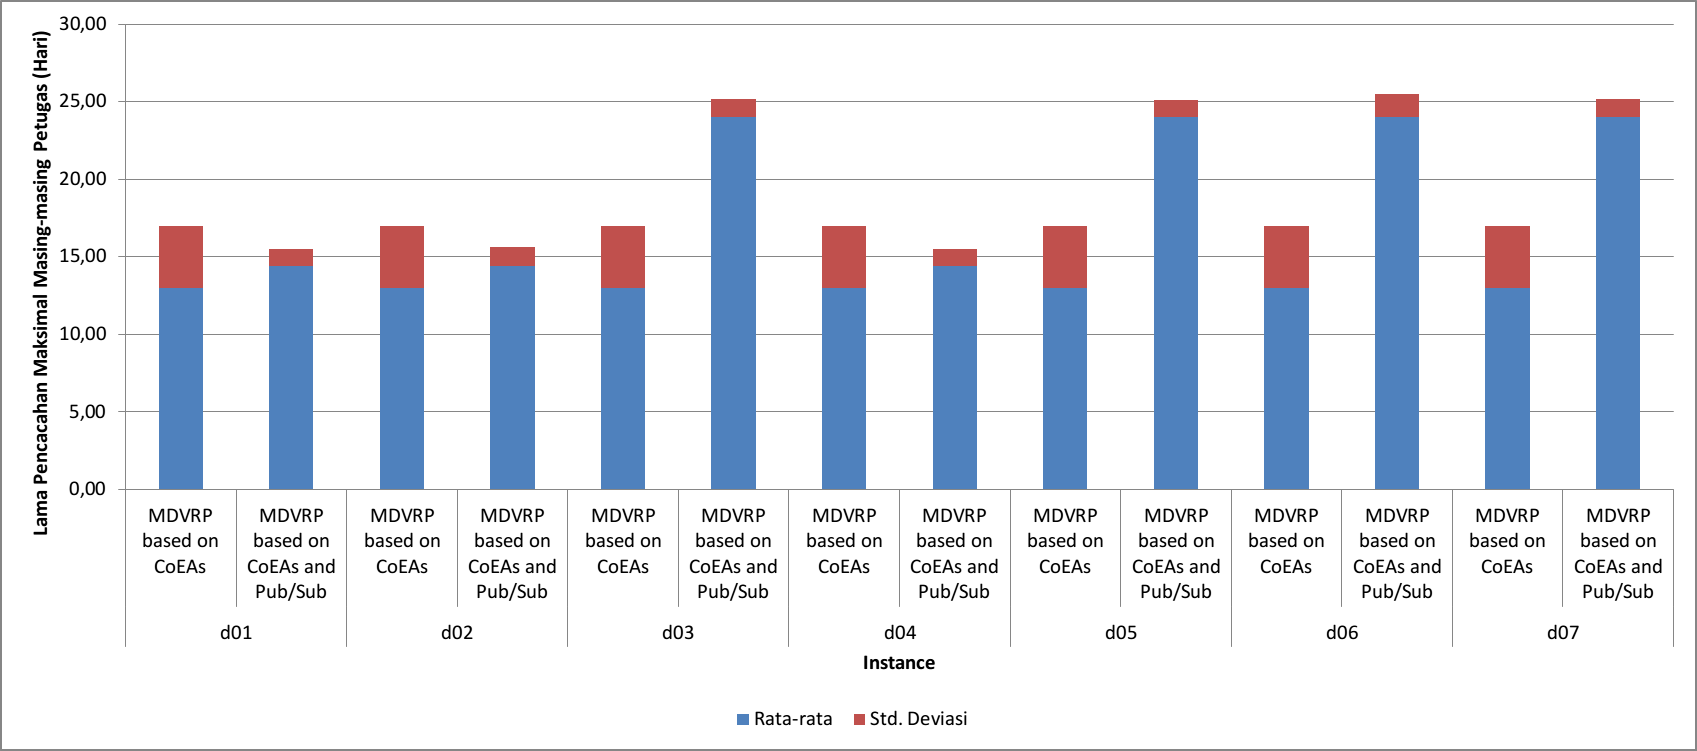
\includegraphics[width=\textwidth]{Resources/Images/test_result_delay_real_tw_mean_stdev_of_total_time}
	\captionsetup{format=hang}
	\caption{Maksimum Lama Pencacahan Masing-masing Petugas (Hari) Dari 100 Pengujian Kondisi Delay dengan Waktu Pencacahan pada Data Lapangan}
	\label{fig:test_result_delay_real_tw_mean_stdev_of_total_time}
\end{figure}



